The performance evaluation is split into two: a shared memory performance
scaling evaluation on a 64 core machine, and a distributed memory performance
evaluation on a cluster on up to 12 nodes.

\subsection{Evaluation Methodology}
\label{sec:mpievaluationmethodology}

The performance evaluation aimed to test the scalability of the parallelised
application in two ways. The first is with a fixed area under test. This will
show how a given problem (150x150x90 in size) would scale in multi-core and
multi-socket machines and in a cluster. The second test is with an expanding
area. This is where, for all runs, each process has its own area of a set size
(150x150x90) such that, as the number of processes grows, the overall
computational area increases at the same rate. This will show how well larger
problem sets can be handled and how the overhead of communication grows as the
number of processes involved in the communication grows.

For a given number of processes, there can be many runs. This is because there
are different ways to lay out the processes in a two dimensional grid. For
instance, the 64 process runs are executed in a 4x16, 8x8, and 16x4 layout. The
quickest layout is reported as the runtime for that number of processes. To
limit the number of configurations, the maximum number of processes in any
single dimension was limited to 16. This limit is for the evaluation only, the
LES supports arbitrarily large process grids.

Many of the graphs, for instance Figure~\ref{fig:mpichfixedarea} have the
occasional spike in runtime. These occur at a prime number of processes. A run
with a prime number of processes will have to have a 1xN or Nx1 layout over the
LES area. This limits the number of neighbours per process to two but, rather
than improving performance due to the reduced number of messages, performance
degrades. This is due to the non-blocking nature of the sends and receives used
in the MPI LES. For other process counts, with up to four neighbours, there is
less work to do for each message exchange meaning the first exchange will start
sooner and have more overlap with subsequent exchanges than the prime number
cases.

\subsection{Shared-memory parallelisation}
The shared-memory parallelisation run was conducted on a machine called togian.
This system is a quad socket AMD Opteron 6366HE system giving it 64 cores paired
into 32 modules running at 1.8GHz. To provide consistent benchmarking results,
the turbo clock frequencies were disabled. The system has been fitted with 512GB
of DDR3 RAM. In terms of software, gfortran version 4.7.2 with MPICH 3.1.3 were
used for the majority of the evaluation. OpenMPI 1.8.4 performance was also
investigated.

\subsubsection{Default Mapping}

The first configuration under evaluation was the default setup for MPICH 3.1.3.
This default mapping assigns processes to cores in a round-robin fashion across
sockets. This spreads the runtime load between CPU sockets thus minimising the
load on the CPUs cache for small numbers of processes and maximises the chance
of achieving a higher turbo clock frequency if applicable.

\begin{figure}
    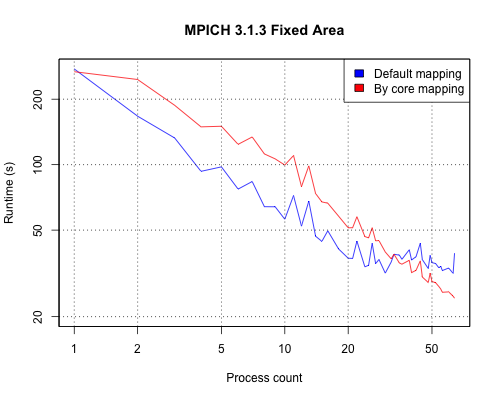
\includegraphics[width=0.5\textwidth]{graphs/MPICH313-fixed-area.png}
    \caption{MPICH 3.1.3 Fixed Area Runtimes}
    \label{fig:mpichfixedarea}
\end{figure}

Figure~\ref{fig:mpichfixedarea} shows linear improvements in runtime for a fixed
sized area. Single threaded performance has a runtime of 275.5 seconds with 64
threads completing its run in 39.2 seconds, a 7x improvement in computational
throughput.

The graph isn't as smooth as would normally be expected. This is as a direct
consequence to the mapping of processes over a two dimensional area. If the same
number of processes exist in both axes, then the performance is at its best
since the length of all halos are equal. If the process counts differ then they
cannot have a balanced layout since two halos will be significantly shorter than
the others. This difference acts as a bottleneck since the shorter halo
exchanges finish sooner then have to wait for the longer halo exchanges to
complete.

Figure~\ref{fig:mpichexpandingarea} shows good scaling of runtime where the
overall area under simulation grows at the same rate as the process count. A
single process executing on a 150x150x90 area takes 69.2 seconds to execute
whereas 64 processes executing on a 1200x1200x90 area takes 235.9 seconds to
execute. This equates to a 3.4x increase in runtime for a 64x increase in area,
improving throughput by 18.8x. Comparing this with the fixed area improvement of
7x, it is clear to see that to get the most benefit from the MPI parallelised
LES, it should be used to to calculate velocities over greater areas or at
greater resolutions than before. This is also as intuition would expect since
the setup cost of sending a message is fixed irrespective of the message size so
larger messages amortize the cost of the setup. Also, as the fixed area runs
gain processes, the ratio between time spent doing useful computation and
message sending decreases.

\begin{figure}
    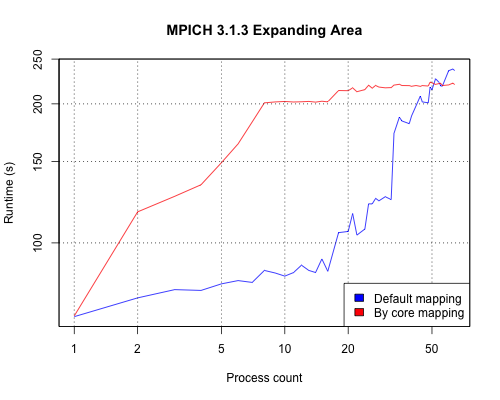
\includegraphics[width=0.5\textwidth]{graphs/MPICH313-expanding-area.png}
    \caption{MPICH 3.1.3 Expanding Area Runtimes}
    \label{fig:mpichexpandingarea}
\end{figure}

Towards the end of the graph there is a significant increase. This occurs on the
move from 32 to 33 processes. This is because at 32 processes, all sockets are
exactly `half full'. Each module has its own hardware thread active so each
process has its own floating point units. On the move to 33 processes, a process
will now have to share floating point units with another process. This will slow
down these processes and, by extension, the application overall. This is a
feature of the AMD CPU architecture and not something caused by MPI or the LES.

\subsubsection{By Core Mapping}

The second configuration under evaluation involved a minor change to MPICH
3.1.3. Instead of using the default mapping of processes to cores, mpiexec was
setup to assign processes to cores sequentially. This means a single socket will
be `filled up' with processes before moving on to the next. The rationale behind
this change was to increase the probability that a processes neighbours were on
the same socket. This is almost always now true for the left and right neighbour
which will be running on the previous and next core respectively. The primary
downsides are increased cache and floating point unit utilisation on smaller
process counts. For example, a four process run is now sharing the resources of
a single socket rather than each having the resources of their own socket.
Another downside is that the turbo frequency will be reduced quicker on
applicable systems since a socket will reach higher process counts sooner.

Figure~\ref{fig:mpichfixedarea} shows that, for the fixed area runs, the
performance difference is negligible. The lower process counts have poorer
performance however, once the 32 process boundary has been crossed, performance
is the same as the default mapping case.

Figure~\ref{fig:mpichexpandingarea} again shows good scaling of
runtime where the overall simulation area increases at the same rate as the
process count increases. It also shows more clearly that runtime levels out so
increases in area are `for free' when increasing the process count by the same
amount. Runtime now levels out at around 220 seconds which is a 7\% improvement
over the default mapping case. This change isn't massive but is consistent and
shows that tweaks outside of the code itself can benefit performance.

As expected, the performance at small process counts is significantly poorer
than in the default mapping case however since it is expected that an entire
shared-memory system or entire nodes would be dedicated to a single application
at any given time this degradation is deemed acceptable given the marginal
performance improvement at higher numbers of processes.

\subsubsection{MPICH versus OpenMPI}

There are two popular implementations of the MPI standard: MPICH and OpenMPI.
Other implementations include several derivatives of MPICH making MPICH one of
the most popular implementations available. OpenMPI is used in many of the
TOP500 supercomputers and is designed to act as an efficient implementation for
common case MPI use cases whereas MPICH acts as a high quality reference
implementation of the latest available MPI standard.

In addition to evaluating performance on MPICH version 3.1.3, the performance
characteristics of OpenMPI version 1.8.4 were also investigated. Many of the
configurations discussed for MPICH were repeated for OpenMPI to enable direct
comparisons between runtimes.

There is no tangible performance difference between MPICH 3.1.3 and OpenMPI
1.8.4. MPICH 3.1.3 is moderately faster but OpenMPI is less than 10\% slower for
high process counts. It can be concluded that use of either MPI implementation
will yield similar speedups as each other. With many other MPI implementations
being based on MPICH, the same performance characteristics could be expected
from those as well.


\subsection{Distributed-memory paralellism}
In addition to shared-memory parallelism, the performance characteristics of the
MPI LES in a distributed-memory environment are of interest. The ability to run
on large computing clusters allows researchers using the LES to simulate at even
higher resolutions or over larger areas than on a single machine.

Results were obtained using the EPSRC funded ARCHIE-WeSt High Performance
Computer (\url{www.archie-west.ac.uk}). EPSRC grant no. EP/K000586/1.

\begin{figure}
    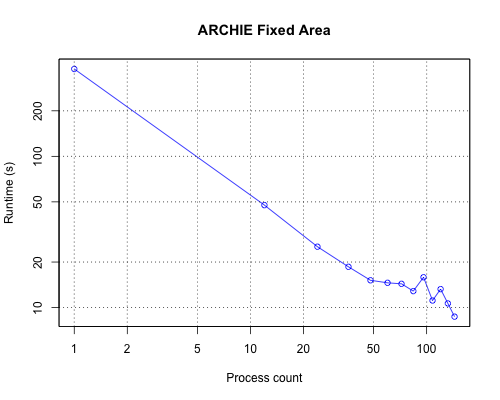
\includegraphics[width=0.5\textwidth]{graphs/ARCHIE-fixed-area.png}
    \caption{ARCHIE Fixed Area}
    \label{fig:archiefixedarea}
\end{figure}

Each node on ARCHIE-WeSt has two Intel Xeon X5650 CPUs. This gives each node 12
cores running at 2.66GHz base frequency. The cluster was setup such that
hyperthreading was disabled but turbo boost was enabled. Each node is fitted
with 48GB RAM and nodes are connected to each other via a 4xQDR Infiniband
Interconnect. ARCHIE's MPI communication library was OpenMPI 1.6.2.

Even though the Intel CPUs have turbo boost enabled, all parallel runs use all
cores of each node so the frequency between runs is consistent.

Figure~\ref{fig:archiefixedarea} shows the performance scaling of a fixed area
problem over 12 nodes (144 cores). For 4 nodes (48 cores) there is good scaling
with 5 to 12 nodes offering only moderate improvements. The single process run
completes in 378.3 seconds. The 4 node run completes in 15.1 seconds and the 12
node run completes in 8.7 seconds. The first 48 cores offer a 25x improvement in
performance with the 144 core run offering a 43.5x improvement. This is expected
as the problem of less useful work per process and increasing communication
costs will ultimately become too great to overcome.

\begin{figure}
    \includegraphics[width=0.5\textwidth]{graphs/ARCHIE-expanding-area.png}
    \caption{ARCHIE Expanding Area}
    \label{fig:archieexpandingarea}
\end{figure}

Figure~\ref{fig:archieexpandingarea} shows the performance scaling of an
expanding area problem over 12 nodes (144 cores). The single core run takes
163.9 seconds. The single node (12 core) run takes 215.5 seconds and the 12 node
run takes 208.9 seconds. Multiple runs of the 12 node run had performance vary
between 207 and 230 seconds, as shown by the error bars. The variation in
runtime between nodes is likely due to the differing load on the cluster
overall. This gives an MPI overhead of around 26.3 to 31.4\%. Crucially, the
runtime does not grow on increasing node count showing the strong scaling
characteristics of the MPI LES.


\subsection{Estimated versus exact corners}

The majority of the communication in the LES involves halo exchanges. These
involve sending and receiving up to four edges between neighbouring processes.
To be mathematically correct, there would also need to be up to four other
communications, a small number of values need to be sent and received for corner
values from four other processes. This brings the total number of messages per
process up to eight. This was thought to be a potential source of overhead,
especially given the overhead of sending a single message was likely to outweigh
the transfers itself. To test this, all runs were repeated with corners instead
being calculated rather than exchanged.

For the shared memory runs, there was a negligible change in performance. This
is likely to be because the cost of calculating floating point units is very
similar to simple memory copies between memory spaces, especially in an AMD
system where floating point units are shared between pairs of cores in what AMD
calls a module.

For the distributed memory runs, exact corners were up to 5\% faster than the
estimated corner runs. The improvement is somewhat more surprising than the
shared memory case however given the fast Infiniband Interconnect between nodes,
the cost of sending a message is likely to be only marginally higher than
communication within a single node. The performance improvement is likely due to
the Xeon X5650's older architecture meaning it supports fewer instruction set
extensions such as AVX and FMA that are known to improve integer and floating
point operation performance.
